% В этом файле следует писать текст работы, разбивая его на
% разделы (section), подразделы (subsection) и, если нужно,
% главы (chapter).

% Предварительно следует указать необходимую информацию
% в файле SETUP.tex

\input{preamble.tex}


\NewBibliographyString{langjapanese}
\NewBibliographyString{fromjapanese}

\begin{document}

\Annot

Результаты, полученные в современной математике, становятся всё сложнее. Постепенно подступает момент, когда математики, работающие в разных областях, окончательно перестанут понимать друг друга, а их результаты станет невозможно проверить. Одним из наиболее активно использующихся решений является проверка математических результатов с помощью средств доказательства теорем. Этот класс инструментов сам по себе заслуживает особого внимания, так как было создано множество непохожих подходов, в основе которых лежат интересные теории.

Гомотопическая теория типов (Homotopy type theory, HoTT) \autocite{hottbook} --- относительно новая область в информатике, которая базируется на неожиданной связи между теорией типов и теорией гомотопий. Эта область лежит в основе \textit{Унивалентных оснований математики} (Univalent Foundation, UF) \autocite{UFP2010} --- попытки формализовать математику, используя в качестве основы не множества, а гомотопические типы или $\infty$-группоиды, а также \textit{высшие индуктивные типы} (Higher Inductive Types, HIT). Этот подход в первую очередь интересен тем, что позволяет работать с гомотопической теорией, используя \textit{синтетический метод}, то есть не опираясь на более базовые примитивы, как, например, множества, также очень важным преимуществом HoTT являются хорошие вычислительные свойства, унаследованные от зависимой теории типов Мартин-Лёфа \autocite{MLTT}. Первоначальная версия гомотопической теории типов включала в себя \textit{аксиому унивалентности}, что открыло возможность для формализации крупного пласта математики на теоретико-типовом языке: экстенсиональности функций и равенства структур, между которыми доказано существование изоморфизма. Но у этой версии было одно очень важное ограничение --- аксиома не имела вычислительной интерпретации. В данный момент наиболее многообещающим решением является использование \textit{кубической теории типов} \autocite{CohenCHM16}, в которой эта аксиома является теоремой, имеющей конструктивное доказательство.

Для обоснования гомотопической интерпретации следует доказать эквивалентность конструкций, которые есть в теории типов, с гомотопическими понятиями. И если гомотопическая интерпретация функций, типов-равенств интуитивно понятна, то зависимые типы требуют большего внимания. В этой работе исследуется доказывательство изоморфизма между $\Pi$-типом и расслоением в системе верификации доказательств Arend. 

Код, которому посвящена данная работа, можно найти на GitHub \autocite{Grp1} в репозитории организации Groupoid Infinity.

\section{Dependent types}

\subsection{Brief preliminaries}

Dependent types can be briefly summarized with a few postulates:
\begin{enumerate}
  \item A hierarchy of type universes is given: $U_0 : U_1 : U_2 : \dots$.
  \item If the universe level is unambiguous, then the level may be dropped.
  \item The statement "$A$ is a type" means that $A : U_i$ for some $i \in \N$.
  \item The statement "$a : A$" is given a meaning, that $a$ is an term of type $A$.
  \item For any types $A$ and $B$, we may form a type $A \to B$ that represents a function. And a term $f : A \to B$ of this type may be constructed by demonstrating that $f(a) : B$ under the assumption $a : A$.
  \item A dependent type is a morphism to the universe $P : A \to U$, so a dependent type $P : A \to U$ provides us with a type $P(a)$ for any $a : A$.
\end{enumerate}

It can be formalized using Arend:

\begin{ListingEnv}[H]
\begin{lstlisting}
\func family (B : \Type) : \Type => B -> \Type
\end{lstlisting}
\end{ListingEnv}

% TODO

\section{Fiber bundles}
\label{sec:fiberbundles}

\subsection{Idea}
A fiber bundle over an object $B$ is simply a an object $E$ paired with a morphism from $E$ to $B$ in which every fibre is isomorphic to a standard fiber $F$ and a fiber of a morphism over a point of $B$ is the collection of elements of $E$ that are mapped by given morphism to this point. It can be viewed as a parameterized family of objects, each "isomorphic" in some way to $F$, where the family is parameterized by points in $B$.

Fiber bundles arise in several diverse fields such as physics (this concept embodies the two central principles of modern physics: the gauge principle and the principle of locality), Lie theory (principal G-bundles) and homotopy theory (they generalize notion of a covering space in homotopy theory, because a covering space is an fiber bundle where the fibers are discrete sets). Also fundamental objects in algebraic topology (fibrations) and algebraic geometry (sheaves) are simply generalized fiber bundles.

\subsection{Definition}

Some definitions are equipped with a corresponding Arend functions or data types.

\begin{mydefinition}[Bundle]
	A bundle over an object $B$ is an object $E$ equipped with a morphism $\phi$ from $E$ to $B$:
	\[
	\begin{diagram}
		\node{E} 
			\arrow{e,t}{\phi} 
		\node{B} 
	\end{diagram}
	\]
	
	\begin{ListingEnv}[H]
	\begin{lstlisting}
\func bundle (B : \Type) : \Type 
	=> \Sigma (E : \Type) (phi : E -> B)
	\end{lstlisting}
	\end{ListingEnv}
\end{mydefinition}

\begin{mydefinition}[Fiber]
	The fiber of a morphism $f : E \to B$ over a point of $B$ is the collection of elements of $E$ that are mapped by $f$ to this point, hence it is the following pullback (or fiber product) of $pt$ and $f$:
	\[
	\begin{diagram}
		\node{E \times \star}
			\arrow{s,t}{}
			\arrow{e,t}{}
		\node{\star} 
			\arrow{s,t}{pt} \\
		\node{E}
			\arrow{e,t}{f} 
		\node{B}
	\end{diagram}
	\]
	\begin{ListingEnv}[H]
	\begin{lstlisting}
\func fiber (E B : \Type) (f : E -> B) (base : B)
	=> \Sigma (x : E) (f x = base)
	\end{lstlisting}
	\end{ListingEnv}
\end{mydefinition}

\begin{mydefinition}[Fiber bundle]
	A fiber bundle over $B$ with standard fiber $F$ is a bundle $\pi$ over $B$ such that, given any global element $x : \star \to B$, the pullback of $E$ along $x$ is isomorphic to $F$.
\end{mydefinition}

\begin{mydefinition}[Trivial fiber bundle]
	The fiber bundle is trivial if $E$ is simply a product $B \times F$ and $\pi$ is the projection map of the first element of $E$.
	\begin{ListingEnv}[H]
	\begin{lstlisting}
\func total (B : \Type) (F : family B) : \Type 
	=> \Sigma (x : B) (F x)

\func trivial (B : \Type) (F : family B) : total B F -> B 
	=> \lam (x : total B F) => x.1
	\end{lstlisting}
	\end{ListingEnv}
\end{mydefinition}

\subsection{Example}

An idea behind the fiber bundle is that it encapsulates the "global twist". Two fiber bundles over a $S_1$ with $[0..1]$ fibers are visualized below and formalized (Arend code for Möbius strip can be found in Appendix A) for clarification. Locally cylinder and Möbius strip are identical, but globally they differ.
% Some information about Hopf-fibrations?

\begin{figure}[H]
\centering
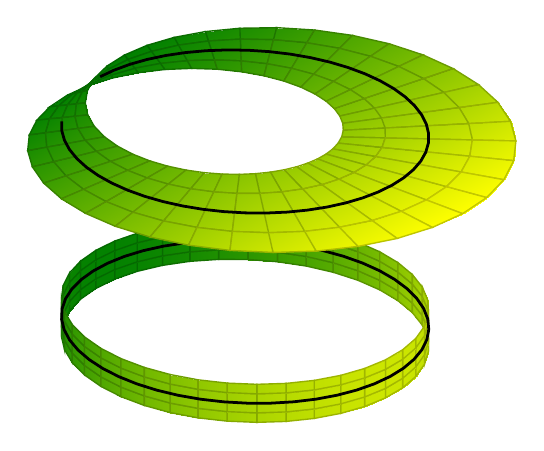
\begin{tikzpicture}[scale=1.25]
\begin{axis}[
    hide axis,
    view={40}{40}
]
\addplot3 [
    surf, shader=faceted interp,
    point meta=x,
    colormap/greenyellow,
    samples=40,
    samples y=5,
    z buffer=sort,
    domain=0:360,
    y domain=-2:2
] (
    {sin(x)},
    {cos(x)},
    {y-20});
\addplot3 [
    samples=50,
    domain=0:360,
    samples y=0,
    thick
] (
    {cos(x)},
    {sin(x)},
    {-20});   
\addplot3 [
    surf, shader=faceted interp,
    point meta=x,
    colormap/greenyellow,
    samples=40,
    samples y=5,
    z buffer=sort,
    domain=0:360,
    y domain=-1:1
] (
    {(1+0.5*y*cos(x/2)))*cos(x)},
    {(1+0.5*y*cos(x/2)))*sin(x)},
    {0.5*y*sin(x/2)});
\addplot3 [
    samples=50,
    domain=-145:180,
    samples y=0,
    thick
] (
    {cos(x)},
    {sin(x)},
    {0}); 
\end{axis}
\end{tikzpicture}
\caption{Fiber bundles over a circle} \label{fig:P1}
\end{figure}

\section{Proof}

% TODO

\Conc

% TODO

\printbibliography[%{}
    heading=bibintoc%
    ,title=Bibliography
]

\appendix
\ifthenelse{\value{worktype} > 1}{%
  \addtocontents{toc}{%
      \protect\renewcommand{\protect\cftchappresnum}{\appendixname\space}%
      \protect\addtolength{\protect\cftchapnumwidth}{\widthof{\appendixname\space{}} - \widthof{Глава }}%
  }%
}{
  \addtocontents{toc}{%
      \protect\renewcommand{\protect\cftsecpresnum}{\appendixname\space}%
      \protect\addtolength{\protect\cftsecnumwidth}{\widthof{\appendixname\space{}}}%
  }%
}

\section{Möebius strip}

\begin{ListingEnv}[H]
\begin{lstlisting}
\func squeezePath {A : \Type} {a a' : A} 
	(p : a = a') (i : I) : a = p @ i 
	=> path (\lam j => p @ meet i j)

\func neg_neg : 
	\Pi (x : I) -> ((inv seg) @ (inv seg @ x)) = x 
	=> \lam x 
	=> ((\lam x 
    	=> (\lam i 
    		=> inv (squeezePath (inv seg) i)) (inv seg @ x)) x)
    # (inv ((\lam x 
    	=> ((\lam x 
    		=> (\lam i 
    			=> inv (squeezePath seg i)) (seg @ x)) x) # seg) x))

\func twist : I = I 
	=> Iso=>Path \new Iso I I neg neg neg_neg neg_neg

\func M : \Pi (x : S1) -> \Type => \lam x => \case x \with {
  | base => I
  | loop i => twist @ i
}

\record Moebius (p1 : S1) {
  \field f1 : M(p1)
}
\end{lstlisting}
\end{ListingEnv}

\end{document}
